% !TeX spellcheck = en_GB

\section{Introduction}\label{Introduction}

\subsection{Motivation}

The starting point of this thesis was to get a command line interface (CLI) tool to automatically generate the 4-tuples $exercise = (grammar,\ word,\ parse\ table,\ derivation\ tree)$, which are used to test if the students have understood the way of working of the CYK algorithm.\\
Various implementations of the Cocke-Younger-Kasami (CYK) algorithm can be found. Nevertheless none of them seemed to meet the easy to use requirements to automatically generate suitable $exercise$s, that afterwards also could be modified as wanted.\\
Additionally the task of finding a clever algorithm to automatically generate $exercise$s with a high chance of being suitable as an exam exercise was added. 

\subsection{Grammar in Chromsky Normal Form}
\begin{DefGrey} \textbf{Grammar}\\
	Let there be a grammar $G=(V,\ \Sigma,\ S,\ P)$ for which the following holds:
	\begin{itemize}
		\item $V$ is a finite set of variables.
		\item $\Sigma$ is an alphabet \textendash~called terminals.
		\item $S$ is the start symbol and $S \in V$.
		\item $P$ is a finite set of rules: $P \subseteq V \times (V \cup \Sigma)^{*}$ \textendash~called productions.
	\end{itemize}
\end{DefGrey}
\noindent Further it is assumed that the productions are more restricted and it holds: $P\ \subseteq\ V \times (V^{2} \cup \Sigma)$. Additionally let there be a word $w \in \Sigma^*$ and a language $L(G)$ of the Grammar $G$. \\
\noindent Regarding further convenience for explaining the following default values are true:
\begin{itemize}
	\item $V = \{A, B, ...\}$
	\item $(V^2 \cup\ \Sigma)^{*}=\{a, b, ...\} \cup \{AB, BS, AC, ... \}$
\end{itemize}
\noindent Moreover in the context of talking about sets, a set is always described beginning with an upper case letter, while one specific element of a set is described beginning with a lower case letter. Example: A "$Pyramid$" is a set consisting of multiple "$Cell$"s, which again is a subset of the set of variables "$V$". A "$cellElement$" is one specific element of a "$Cell$". (For further reasoning behind this example see chapter XXX "help data structure") 
\pagebreak
\subsection{General approaches}
Two basic approaches, that may help finding a good algorithm are explained informally.
\subsubsection{Forward Problem \& Backward Problem}
The Forward Problem and the Backward Problem are two ways as how to determine if $w \in L(G)$.	
\begin{DefGrey}
	\textbf{Forward Problem ($G \xrightarrow[]{derivation} w$)} \\
	Input: Grammar $G$ in CNF. \\
	Output: Derivation $d$ that shows implicitly $w \subseteq L$.
\end{DefGrey}
\noindent It is called Forward Problem, if you are given a grammar $G$ and form a derivation from its root node to a final word $w$. The final word $w$ is always element of $L(G)$.
\begin{DefGrey}
	\textbf{Backward Problem = Parsing ($w\overset{?}{\subseteq}L(G)$)}\\
	Input: $w$ and a grammar $G$ in CNF. \\
	Output: $w \subseteq L(G) \Longrightarrow$ derivation $d$.
\end{DefGrey}
\noindent It is called Backward Problem, if you are given a word $w$ and want to determine if it is element of $L(G)$. "This process, called parsing, is virtually always much more difficult than forming a derivation."
\subsubsection{Parsing Bottom-Up \& Top-Down}
There are again two ways of how the approach of parsing can be classified.
\begin{DefGrey}
	\textbf{Bottom-Up} \\
	 Bottom-Up parsing means to start parsing from the leaves up to the root node.
\end{DefGrey}
\noindent "Bottom-Up parsing is the general method used in the Cocke-Younger-Kasami(CYK) algorithm, which fills a parse table from the "bottom up"."[Duda 8.6.3 page 426]
\begin{DefGrey}
	\textbf{Top-Down} \\
	 Top-Down parsing means to start parsing from the node down to the leaves.
\end{DefGrey}
\noindent Top-Down parsing means to start parsing from the node down to the leaves. "Top-Down parsing starts with the root node and successively applies productions from $P$, with the goal of finding a derivation of the test sentence $w$. Because it is rare indeed that the sentence is derived in the first production attempted, it is necessary to specify some criteria to guide the choice of which rewrite rule to apply. Such criteria could include beginning the parse at the first (left) character in the sentence (i.e., finding a small set of rewrite rules that yield the first character), then iteratively expanding the production to derive subsequent characters, or instead starting at the last (right) character in the sentence." [Duda 8.6.3 page 428]\\

\subsection{Data Structure Pyramid}

To be able to describe the way of working of the different algorithms better the help data structure $Pyramid$ will be defined. But before that let there be:
\begin{DefGrey} \textbf{$[i, j]$} \\
	$[i,\ j] := \{i,\ i+1,..., j-1,\ j\} \subseteq \mathbb{N}_{\geq 0}$.
\end{DefGrey}
\noindent Think about if Cellij can be defined as either subset of V or (V,k)
\begin{DefGrey} \textbf{$Cell_{i,j}$} \\
	$Cell_{i,j} \subseteq V$
\end{DefGrey}
\noindent With help of this $Pyramid$ can be defined as following:
\begin{DefGrey} \textbf{$Pyramid$} \\
	$Pyramid :=\{ Cell_{i,j}\ |\ i \in [0,\ i_{max}],\  j \in [0,\ j_{max}-i],\ i_{max} = j_{max} = |word|-1\}$.
\end{DefGrey}
\noindent A $Pyramid$ is called $EmptyPyramid \Leftrightarrow \forall i\ \forall j\ Cell_{i,j}=\emptyset$. \noindent The following is the visual representation of the $Pyramid$:
\newcommand{\boxpyramid}[1]{
	\fontsize{5}{12}\selectfont{#1}
}
\begin{figure}[H]
\centering
	\resizebox{\linewidth}{!}{
		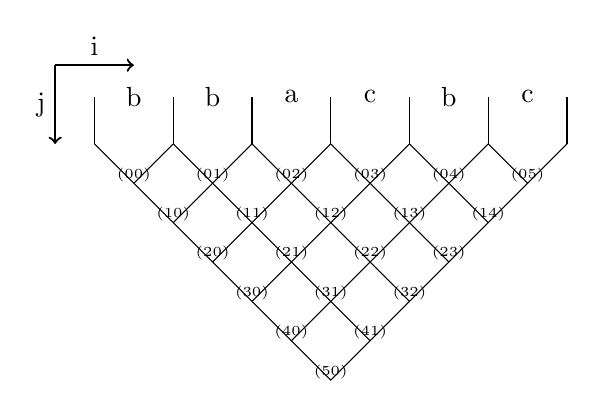
\begin{tikzpicture}[baseline]
		\newcommand{\myfontvars}[1]{
			\fontsize{4.9}{12}\selectfont{#1}
		}\newcommand{\myfontnumbering}[1]{
			\fontsize{2.5}{12}\selectfont{#1}
		}%Outer hull
		%Tip of the pyramid
		\coordinate (tip) at (3,-3);
		\foreach \i in {0,...,6} {
			\coordinate (\i) at (\i,0);
		}
		%\draw[help lines] (-1,1) grid (6,-3);
		\draw [->, thick] (-0.5,1) -- (0.5,1);
		\node [above] at (0, 1) {i};
		\draw [->, thick] (-0.5,1) -- (-0.5,-0.0);
		\node [left] at (-0.5,0.5) {j};
		%Draw the left and right line of the pyramid pointing downwards
		\draw (0) -- (tip) -- (6);
		%Grid lines direction down-left to top-right
		\coordinate (dl1) at (0.5,-0.5);
		\coordinate (dl2) at (1.0,-1.0);
		\coordinate (dl3) at (1.5,-1.5);
		\coordinate (dl4) at (2.0,-2.0);
		\coordinate (dl5) at (2.5,-2.5);
		\draw (dl1) -- (1,0);
		\draw (dl2) -- (2,0);
		\draw (dl3) -- (3,0);
		\draw (dl4) -- (4,0);
		\draw (dl5) -- (5,0);
		%Grid lines direction down-right to top-left
		\coordinate (dr1) at (3.5,-2.5);
		\coordinate (dr2) at (4.0,-2.0);
		\coordinate (dr3) at (4.5,-1.5);
		\coordinate (dr4) at (5.0,-1.0);
		\coordinate (dr5) at (5.5,-0.5);
		\draw (dr1) -- (1,0);
		\draw (dr2) -- (2,0);
		\draw (dr3) -- (3,0);
		\draw (dr4) -- (4,0);
		\draw (dr5) -- (5,0);
		%Small lines at the top
		\coordinate (top0) at (0.0,0.0);
		\coordinate (top1) at (1.0,0.0);
		\coordinate (top2) at (2.0,0.0);
		\coordinate (top3) at (3.0,0.0);
		\coordinate (top4) at (4.0,0.0);
		\coordinate (top5) at (5.0,0.0);
		\coordinate (top6) at (6.0,0.0);
		\coordinate (topUpper0) at (0.0,0.6);
		\coordinate (topUpper1) at (1.0,0.6);
		\coordinate (topUpper2) at (2.0,0.6);
		\coordinate (topUpper3) at (3.0,0.6);
		\coordinate (topUpper4) at (4.0,0.6);
		\coordinate (topUpper5) at (5.0,0.6);
		\coordinate (topUpper6) at (6.0,0.6);
		\draw (top0) -- (topUpper0);
		\draw (top1) -- (topUpper1);
		\draw (top2) -- (topUpper2);
		\draw (top3) -- (topUpper3);
		\draw (top4) -- (topUpper4);
		\draw (top5) -- (topUpper5);
		\draw (top6) -- (topUpper6);
		%The string
		\coordinate (w0) at (0.5,0.6);
		\coordinate (w1) at (1.5,0.6);
		\coordinate (w2) at (2.5,0.6);
		\coordinate (w3) at (3.5,0.6);
		\coordinate (w4) at (4.5,0.6);
		\coordinate (w5) at (5.5,0.6);
		\node [] at (w0) {b};
		\node [] at (w1) {b};
		\node [] at (w2) {a};
		\node [] at (w3) {c};
		\node [] at (w4) {b};
		\node [] at (w5) {c};
		% Variables in the cells
		%cell00
		\coordinate (center00) at (0.5,0.0);
		\node [below=0.18cm] at (center00) {\myfontnumbering{$(00)$}};
		%cell01
		\coordinate (center01) at (1.5,0.0);
		\node [below=0.18cm] at (center01) {\myfontnumbering{$(01)$}};
		%cell02
		\coordinate (center02) at (2.5,0.0);
		\node [below=0.18cm] at (center02) {\myfontnumbering{$(02)$}};
		%cell03
		\coordinate (center03) at (3.5,0.0);
		\node [below=0.18cm] at (center03) {\myfontnumbering{$(03)$}};
		%cell04
		\coordinate (center04) at (4.5,0.0);
		\node [below=0.18cm] at (center04) {\myfontnumbering{$(04)$}};
		%cell05
		\coordinate (center05) at (5.5,0.0);
		\node [below=0.18cm] at (center05) {\myfontnumbering{$(05)$}};
		%cell10
		\coordinate (center10) at (1.0,-0.5);
		\node [below=0.18cm] at (center10) {\myfontnumbering{$(10)$}};
		%cell11
		\coordinate (center11) at (2.0,-0.5);
		\node [below=0.18cm] at (center11) {\myfontnumbering{$(11)$}};
		%cell12
		\coordinate (center12) at (3.0,-0.5);
		\node [below=0.18cm] at (center12) {\myfontnumbering{$(12)$}};
		%cell13
		\coordinate (center13) at (4.0,-0.5);
		\node [below=0.18cm] at (center13) {\myfontnumbering{$(13)$}};
		%cell14
		\coordinate (center14) at (5.0,-0.5);
		\node [below=0.18cm] at (center14) {\myfontnumbering{$(14)$}};
		%cell20
		\coordinate (center20) at (1.5,-1.0);
		\node [below=0.18cm] at (center20) {\myfontnumbering{$(20)$}};
		%cell21
		\coordinate (center21) at (2.5,-1.0);
		\node [below=0.18cm] at (center21) {\myfontnumbering{$(21)$}};
		%cell22
		\coordinate (center22) at (3.5,-1.0);
		\node [below=0.18cm] at (center22) {\myfontnumbering{$(22)$}};
		%cell23
		\coordinate (center23) at (4.5,-1.0);
		\node [below=0.18cm] at (center23) {\myfontnumbering{$(23)$}};
		%cell30
		\coordinate (center30) at (2.0,-1.5);
		\node [below=0.18cm] at (center30) {\myfontnumbering{$(30)$}};
		%cell31
		\coordinate (center31) at (3.0,-1.5);
		\node [below=0.18cm] at (center31) {\myfontnumbering{$(31)$}};
		%cell32
		\coordinate (center32) at (4.0,-1.5);
		\node [below=0.18cm] at (center32) {\myfontnumbering{$(32)$}};
		%cell40
		\coordinate (center40) at (2.5,-2.0);
		\node [below=0.18cm] at (center40) {\myfontnumbering{$(40)$}};
		%cell41
		\coordinate (center41) at (3.5,-2.0);
		\node [below=0.18cm] at (center41) {\myfontnumbering{$(41)$}};
		%cell50
		\coordinate (center50) at (3.0,-2.5);
		\node [below=0.18cm] at (center50) {\myfontnumbering{$(50)$}};
		\end{tikzpicture}
	}
\caption{Visual representation of the pyramid}
\end{figure}
\begin{DefGrey} \textbf{$CellDown,~CellUpperLeft~and~CellUpperRight$} \\
	Let there be a $Cell_{i,j}$. It holds $CellDown = Cell_{i,j}$. \\
	So there are $CellUpperLeft = Cell_{i-1,j}$ and $CellUpperRight = Cell_{i-1,j+1}$.
\end{DefGrey}

\pagebreak
\subsection{ Cocke-Younger-Kasami CYK}


\frame{
	\begin{algorithm}[H] %or another one check
		\caption{CalculateSubsetForCell}
		\label{CalculateSubsetForCell}
		\SetAlgoLined
		\KwIn{$cell_ {i,j} \in pyramid $}
		\KwOut{$V_{i,j} \subseteq V^2$}
		$V_{i,j} = \emptyset $\;
		\For{$k:=i-1 \to 0$}{
			$V_{i,j} = V_{i,j} \cup \{X\ |\ X\longrightarrow YZ,\ Y \in V_{k,j},\ Z \in V_{i-k-1,k+j+1} \}$\;
		}
		
		\Return $V_{i,j}$\;
	\end{algorithm}
}
Algorithm \ref{CalculateSubsetForCell} describes the magic of the CKY-algorithm. It shows what cells are taken into account while filling one cell of the parse table.

\pagebreak
\subsection{Success Rates}
\noindent The Success Rates ($SR$) are used to compare the algorithms accounting to their performance of the different requirements. Let $N$ be the overall count of all generated grammars of the examined algorithm.\\

\noindent Write down if the cellsVar or the cellsVarK are used.\\
Mention the basic connection between the success rates.\\
Write down the default values used for this.\\


\noindent\textbf{Overall Success Rate}
An generated $exercise$ contributes to the Overall Success Rate ($SR$) iff it contributes to the Success Rate Producibility ($SRP$), to the Success Rate Grammar Constraints ($SRG$) and to the Success Rate Pyramid Word Constraints ($SRPW$) at the same time.\\
It holds: $SR = n / N$, whereas $n$ is the count of $exercises$ that fulfil the requirements in this case.\\

\noindent\textbf{Success Rate Producibility}
An generated $exercise$ contributes to the $SRP$ iff the CYK algorithm's output is true.\\
It holds: $SRP = p / N$, whereas $p$ is the count of $exercises$ that fulfil the requirements in this case.\\

\noindent\textbf{Success Rate Grammar Constraints}
An generated $exercise$ contributes to the $SRG$ iff the following conditions are met:
\begin{itemize}
	\item grammar has got less than a certain amount of productions.
\end{itemize}
It holds: $SRG = g / N$, whereas $g$ is the count of $exercises$ that fulfil the requirements in this case.\\

\noindent\textbf{Success Rate Word Pyramid Constraints}
An generated $exercise$ contributes to the $SRWP$ iff the following conditions are met:
\begin{itemize}
	\item A certain amount of cells force a right cell combination.
	\item There are less than a certain amount of variables in the entire pyramid.
	\item There are less than a certain amount of variables in each cell of the pyramid.
\end{itemize}
It holds: $SRWP = wp / N$, whereas $wp$ is the count of $exercises$ that fulfil the requirements in this case.
\pagebreak

\noindent Fore more detail of fore right cell combination see here:\\

\noindent 
\frame{
	\begin{algorithm}[H] %or another one check
		\caption{checkForceCombinationPerCell}
		\label{checkRightCellPerCombination}
		\SetAlgoLined
		\KwIn{$ CellDown\subseteq V,\ CellUpperLeft\subseteq V,\ CellUpperRight \subseteq V,\ P \subseteq V \times (V^{2} \cup \Sigma) $ }
		\KwOut{$true \iff at~least~one~variable~forces$}
		$VarsForcing \subseteq V$\;
		$VarComp = \{xy\ |\ x \in CellUpperLeft\ \wedge\ y \in CellUpperRight \}$\;
		\ForEach{$v \in CellDown$}{
			$Prods = \{p\ |\ p \in P\ \wedge\ p=(v_1,rhse_1)\ \wedge\ v==v_1 \}$\;
			$Rhses = \{rhse\ |\ p \in Prods\ \wedge\ p=(v_1,rhse_1)\ \wedge\ rhse==rhse_1\} $\;
			\If{$Rhses \nsubseteq VarComp$}{
				$VarsForcing = VarsForcing \cup v$\;
			}			
		}
		\Return $|VarsForcing| > 0$\;
		\footnotetext{
		}
	\end{algorithm}
}


\pagebreak